% (4 Seiten)
\section{Evaluation of the Classification Models}
\label{sec:ModelEval}
This section first evaluates different classification models with three quality measures. These are the precision $P$, the recall $R$ and the $F_{\beta}$-score, which are defined in Definition \ref{def_prf}. Specifically, the $F_1$-score is used, which is the harmonic mean of the precision and the recall and thus favors neither. Then the class thresholds of a Random Forest model is evaluated to see whether or not it can be used to create both a high precision and a high recall model to create seed and candidate alignments as described by Grütze et al.\ \cite{coheel}. These quality measures are unrealistic for the use case of this approach as they do not take the collisions described in Section \ref{sec:NEL} into account. That's why they will be compared with adjusted quality measures, which take the collisions into account, at the end of this section.\par
Let $T$ be the set containing the feature entries to be classified. Each feature entry has a label containing the result (positive or negative) the classifier should predict. A positive label on a feature entry means that its alias links to its entity and that it should be classified as such. A negative label means that the feature entry should not be classified as links because either it's not a link at all or it links to the wrong entity. The subsets $T_{TP}$, $T_{FP}$ and $T_{FN}$, which are used to calculate the quality measures, are defined as follows.\\
\begin{nscenter}
	$T_{TP} \subset T$, where $\forall f_e \in T_{TP}: f_e$ is labeled positive $\land$ $f_e$ is classified positive\\
	$T_{FP} \subset T$, where $\forall f_e \in T_{FP}: f_e$ is labeled negative $\land$ $f_e$ is classified positive\\
	$T_{FN} \subset T$, where $\forall f_e \in T_{FN}: f_e$ is labeled positive $\land$ $f_e$ is classified negative\\
\end{nscenter}
\begin{definition}
$P = \frac{\abs{T_{TP}}}{\abs{T_{TP} \ \cup \ T_{FP}}}$
$R = \frac{\abs{T_{TP}}}{\abs{T_{TP} \ \cup \ T_{FN}}}$
$F_{\beta} = \frac{(1 \ + \ \beta^2) \ \cdot \ P \ \cdot \ R}{(\beta^2 \ \cdot \ P) \ + \ R}$
\label{def_prf}
\end{definition}
% precision, recall reference: Cleverdon, C.W., Mills, J., and Keen, E.M. (1966). An inquiry in testing of information retrieval systems. (2 vols.). Cranfileld, U.K.: Aslib Cranfield Research Project, College of Aeronautics.
\subsection{Model Comparison}
The following classification models are tested: Naive Bayes, Logistic Regression, Gradient Boosted Trees and Random Forest. The implementations of the Apache Spark MLlib \footnote{https://spark.apache.org/mllib/} will be used. Specifically, the Data Frame API of Spark 2.1.0, since it is the primary API. If parameters of a model are not discussed further, then the default parameters of the Spark  MLlib were used. The data set used to train and test the models is extracted from the Wikipedia pages $W_{bsn}$ as described in Section \ref{sec:NEL}. 70\% of the generated feature entries are used to train the model and the remaining 30\% are used to test it. Since the data set contains many more negative entries than positive entries, it is very likely for a model to classify every feature entry as negative. That way the model would still have an accuracy of over 99\%. To mitigate this, the training set is filtered by removing each entry having a rank $\geq 10$. This rank is the higher order feature of either the link score or the context score.\par
Figure \ref{classifier_eval} shows precision, recall, $F_1$-score and $F_{0.25}$-score of the four tested models. Both the Naive Bayes and the Logistic Regression classified every feature entry as negative, which resulted in a precision, $F_1$-score and $F_{0.25}$-score of NaN (due to the division by 0). This is caused by too many negative input feature entries with not enough positive ones as just described. Contrary to them, both the Gradient Boosted Trees and the Random Forest classified the data successfully. Only these two models use Decision Trees, showing that such unequal distributions of negative and positive input data are handled better by Decision Tree based models. The results of both are very similar, with the Random Forest having 2\% more precision and the Gradient Boosted Trees having 6\% more recall. The focus lies on the reliability of the model and thus on the precision. Because of that the $F_{0.25}$-score, which favors the precision and thus mirrors the wanted reliability of them models, is displayed as well. It displays that the Random Forest performs better when the precision is emphasized. It is, therefore, used for the feature evaluation in Section \ref{sec:FeatureEval}.\par
Most models have class thresholds as parameters as well. With these, a class can be favored. The thresholds can be set to either favor the class positive or the class negative. In the case of favoring the class negative, the classifier needs to be more certain about a feature entry to classify it as a link. In the opposite case of favoring the class positive, the classifier needs to be less certain and thus classifies many more feature entries as a link.\par
\begin{figure}[H]
	\centering
	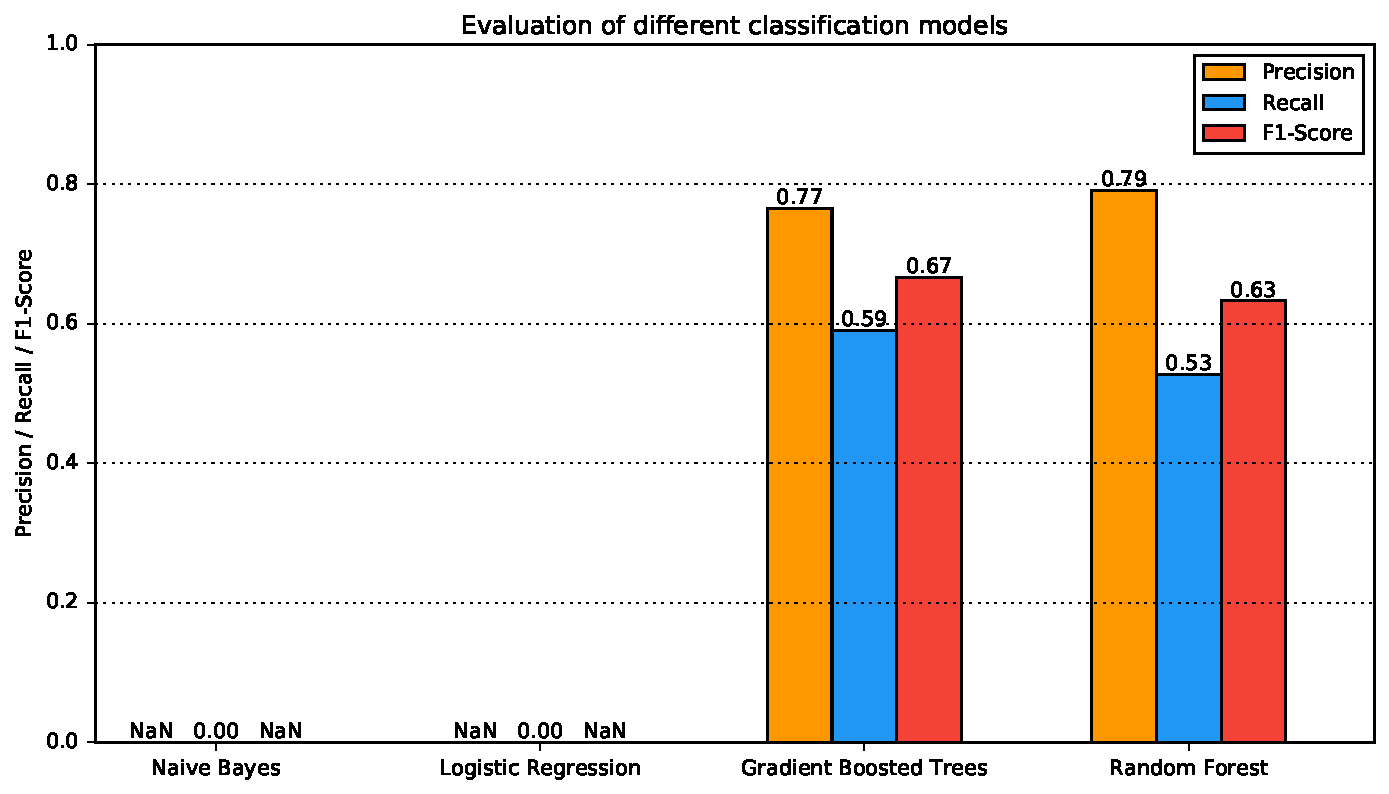
\includegraphics[width=0.9\textwidth]{img/classifier_eval}
	\caption{Evaluation of different classification models.}
	\label{classifier_eval}
\end{figure}
The Naive Bayes and Logistic Regression were both tested with different thresholds for the classes. They were especially tested with thresholds heavily favoring the positive class to see whether or not they would classify anything as positive. Unfortunately, this did not result in a different classification result.\par
The same parameters concerning the Decision Trees were used for the Gradient Boosted Trees and the Random Forest. These were 20 trees, a maximum depth of 6 and a maximum of 40 bins. The Gradient Boosted Trees were tested with a few different number of iterations. The values displayed in Figure \ref{classifier_eval} were the best for the tested number of iterations, which were 20. The other values resulted in a minimally worse precision. The number of trees, the maximum depth and the maximum number of bins were tested using a Random Forest, but none of these parameters changed anything significantly.\par

\subsection{Class Threshold Evaluation}
The class thresholds can be, as previously described, used to favor one class over the other. Since the Spark MLlib does not provide a way to change the class thresholds or the loss function for Gradient Boosted Trees the evaluation of the class thresholds was done only with a Random Forest. Figure \ref{rf_thresh_large} shows the behavior of the quality measures with a different threshold. A threshold $> 1$ means that the class positive is favored and a threshold $< 1$ means that the class negative is favored. The relative distance signifies how strong a class is favored, i.e., a threshold of $0.5$ favors the class negative as much as a threshold of $2.0$ favors the class positive.\par
\begin{figure}[H]
	\centering
	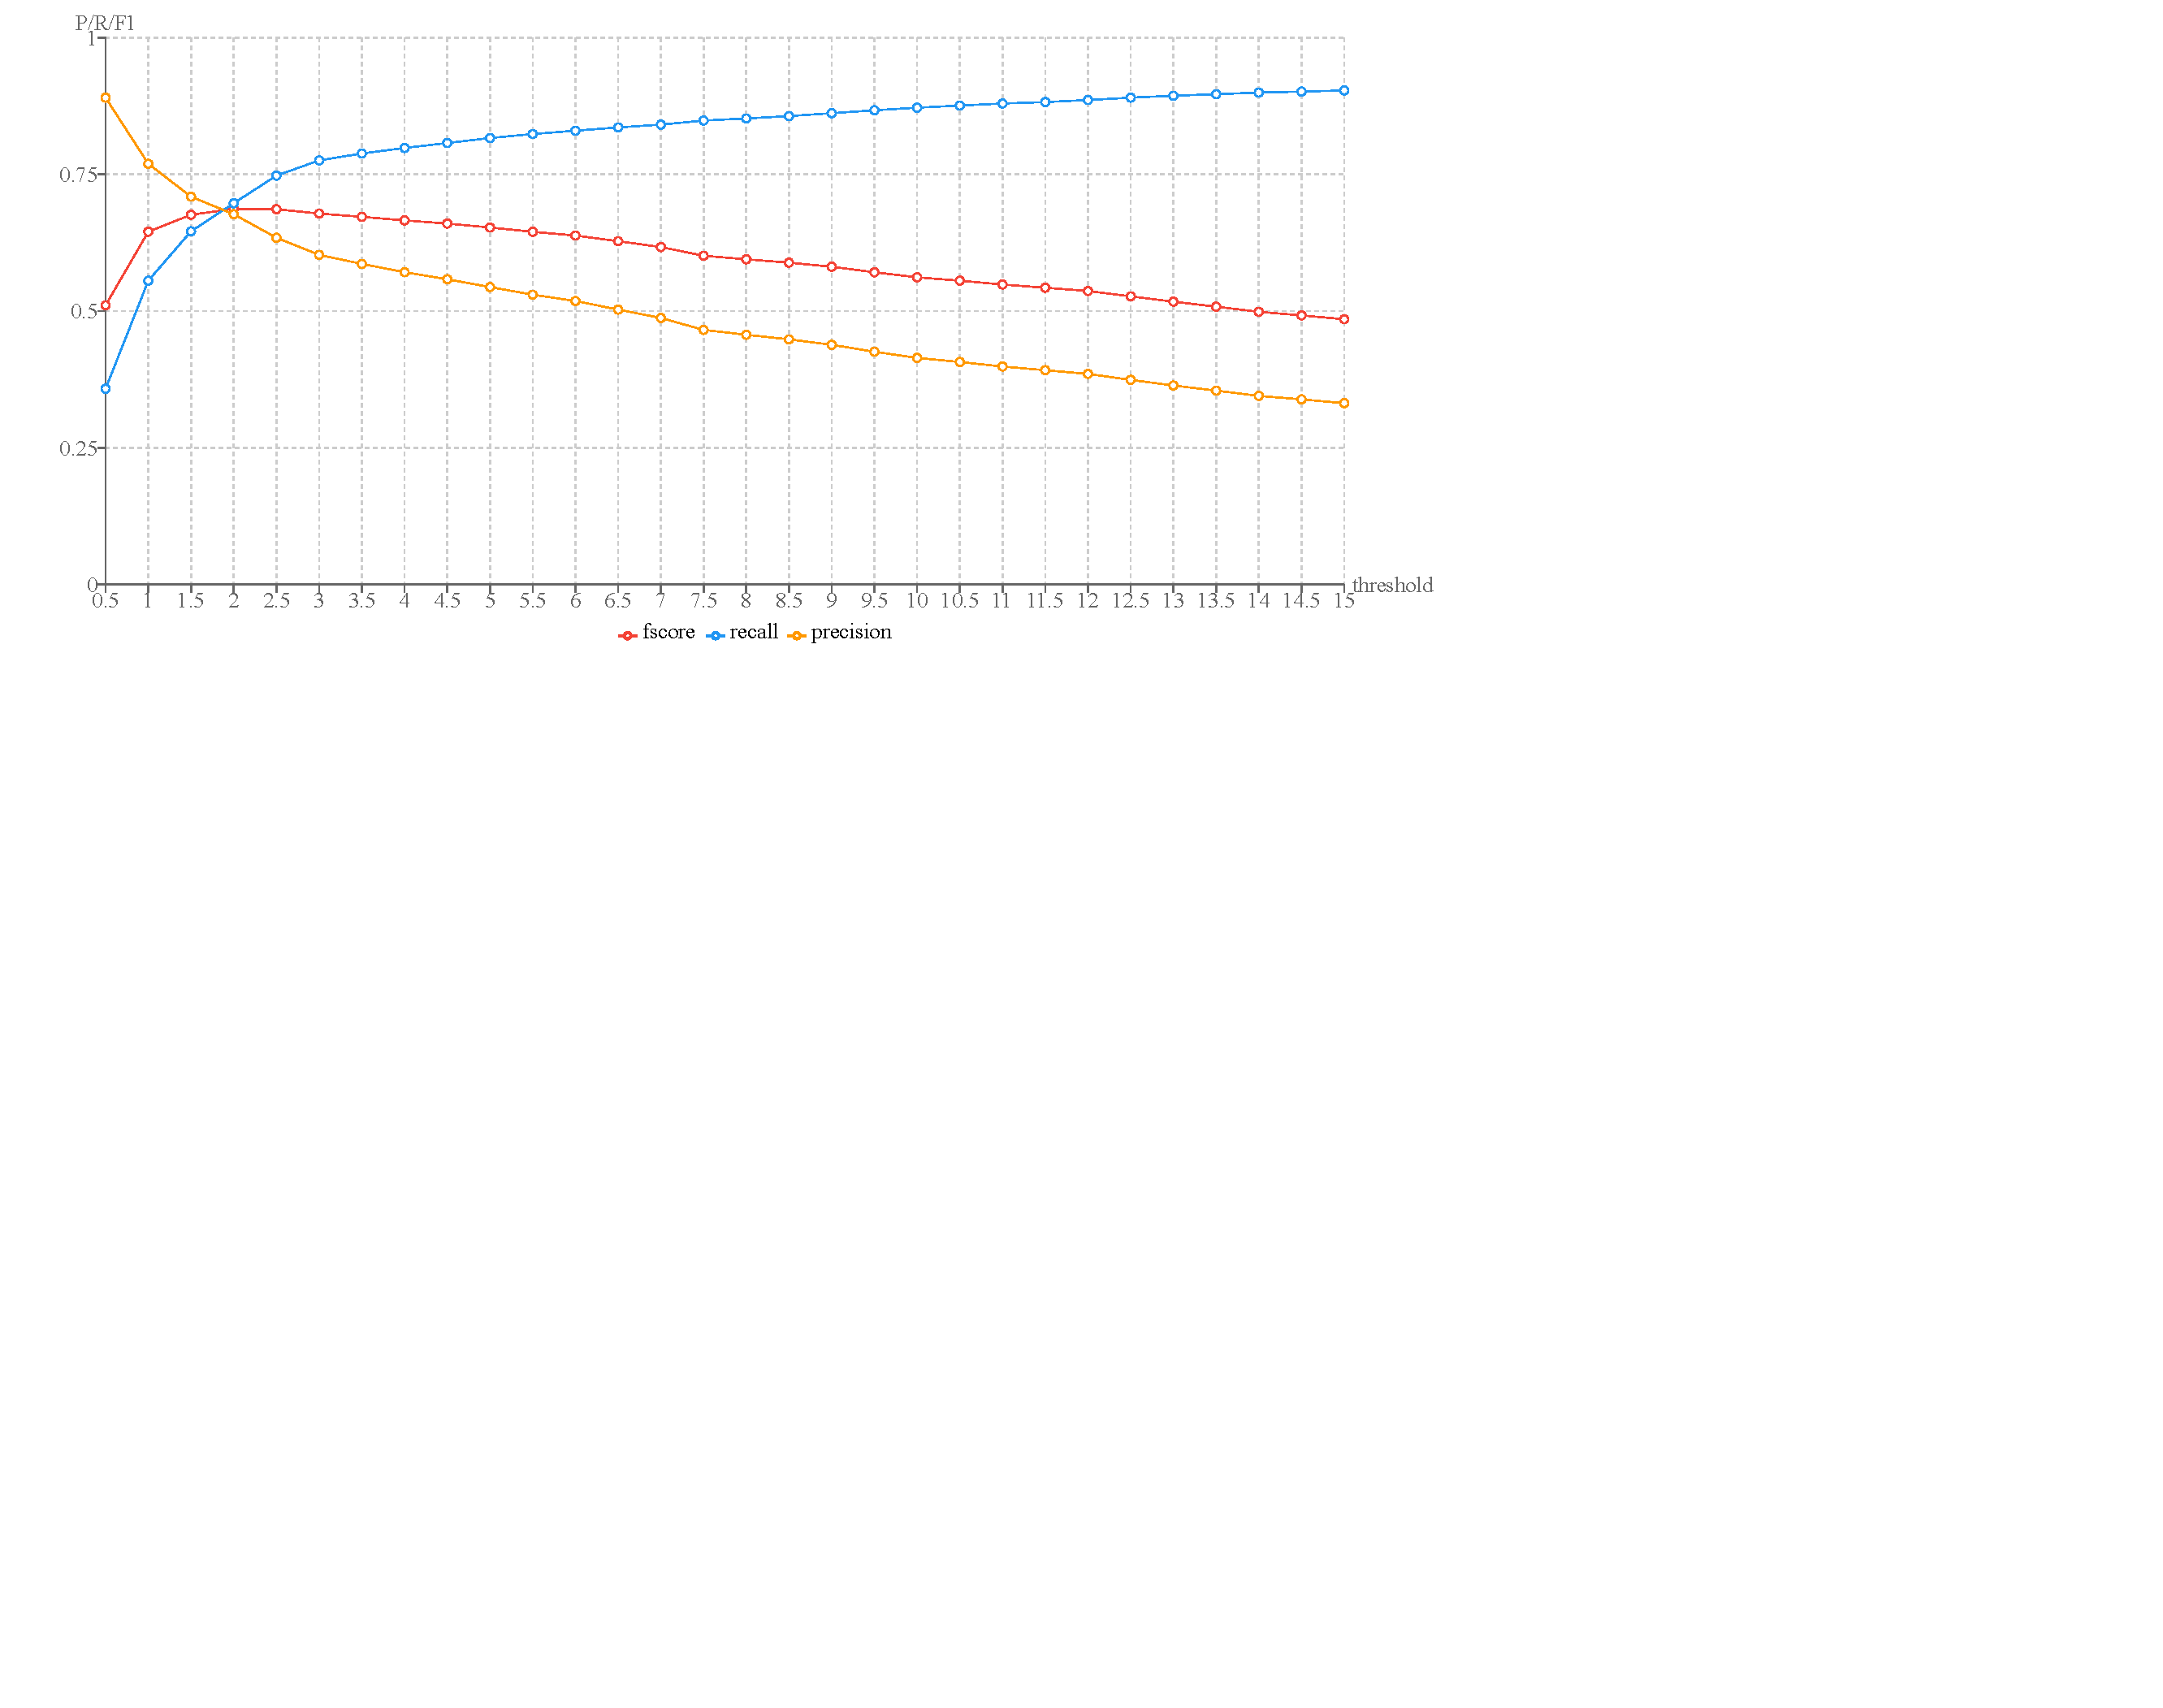
\includegraphics[width=0.9\textwidth]{img/rf_thresh_large}
	\caption{Evaluation of different class thresholds of a random forest model.}
	\label{rf_thresh_large}
\end{figure}
It is visible that a low threshold results in a very high precision with a relatively low recall. The threshold of $0.5$ results in a precision of $89\%$ and a recall of $36\%$. A very high threshold leads to a higher recall with a worse precision. An $80\%$ recall is achieved with a threshold of $4$, which has a precision of $57\%$. A $90\%$ recall is achieved with a threshold of $14.5$, which has a precision of $34\%$. This shows that increasing the threshold has diminishing returns for the recall while the drop of the precision is relatively uniform.\par
Adjusting the thresholds indeed produces a high precision and a high recall classifier, which in the future can be used to create the high-quality seed and high-coverage candidate alignments presented by Grütze et al.\ \cite{coheel}. The candidate alignments would be used to increase the recall of the seed alignments, e.g., by using Random Walks.\par

\subsection{Comparison with realistic Quality Measures}
The adjusted quality measures take the collisions described in Section \ref{sec:NEL} into account. These are an adjusted precision and an adjusted recall. They are calculated the same way the normal precision and recall are calculated but use different sets for the calculation.\par
Let the set $U \subset T$ contain all feature entries, which were the only ones classified as positive for its alias, i.e., there is no collision. $U$ is then used to remove all feature entries with collisions. Let $T'_{TP} = T_{TP} \cap U$ and $T'_{FP} = T_{FP} \cap U$. The feature entries producing collisions are then added to $T_{FN}$: $T'_{FN} = T_{FN} \cup (T_{TP} - U) \cup (T_{FP} - U)$. The sets $T'_{TP}$, $T'_{FP}$ and $T'_{FN}$ are then used to calculate precision, recall and $F_1$-score.\par
\begin{figure}[H]
	\centering
	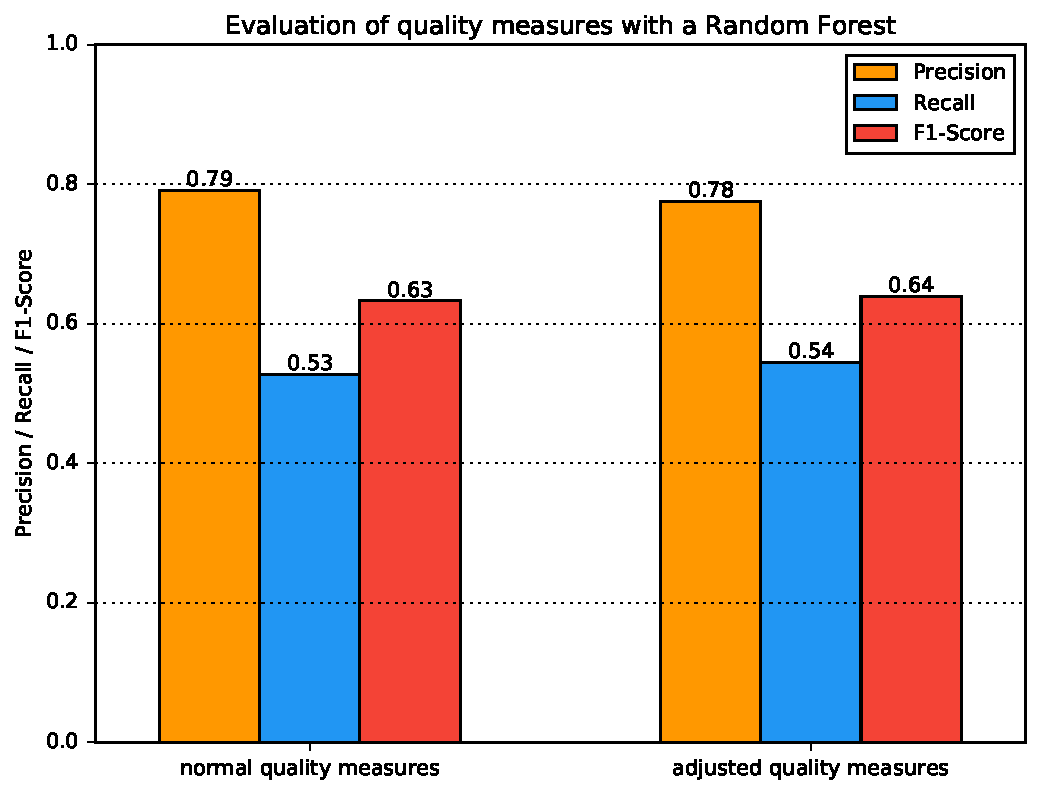
\includegraphics[width=0.7\textwidth]{img/qualitymeasure_eval}
	\caption{Evaluation of quality measures.}
	\label{qualitymeasure_eval}
\end{figure}
Figure \ref{qualitymeasure_eval} shows that, while taking the collisions into account, the precision drops only by one per cent. This proves that the classifier does not produce a lot of collisions and, therefore, the original quality measures are accurate enough to properly evaluate the classification models in this section and the features in the next section.
